\chapter{Metodologia}
\label{cap:5}

Per a desenvolupar aquest treball, s'ha seguit una metodologia similar al tipus \textit{waterfall}, que és un enfocament seqüencial en el desenvolupament de projectes. En aquest model, cada fase es completa abans de passar a la següent. S'ha escollit perquè és molt adient per a projectes unipersonals com aquest.

S'han seguit fases diferenciades, ben definides i amb objectius clars, on només es perseguien els objectius marcats en aquella fase, amb l'excepció de la documentació, que s'ha anat generant i recopilant durant tota l'elaboració del treball.Per a cada fase, s'ha acordat amb el tutor el moment en què caldria tornar a reunir-se per solucionar dubtes i encarar la següent fase. Durant l'elaboració de les fases, també s'han anat plantejant i resolent dubtes, tant sobre el projecte en concret com sobre els treballs de final de grau en general.

Finalment, cal comentar que la intenció principal a l'hora de plantejar el treball ha estat sempre tenir en compte el temps limitat disponible per a desenvolupar-lo. En conseqüència, s'ha buscat l'essència del projecte per tal que el treball sigui el més breu i concís possible, centrant-se en l'anàlisi, que al cap i a la fi és l'objectiu principal del treball.


\begin{figure}[!htbp] 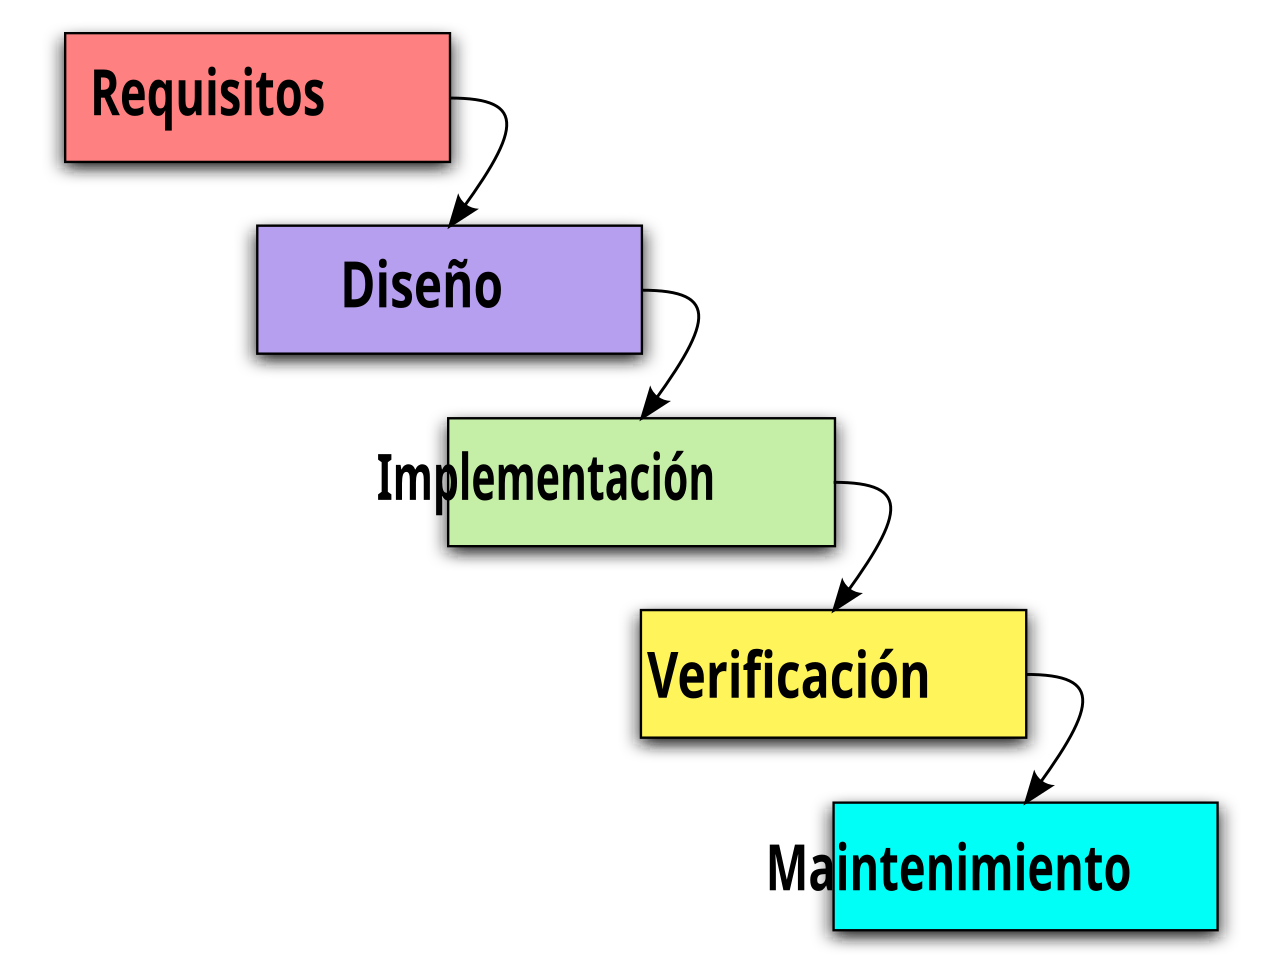
\includegraphics[width=0.5\textwidth]{Imatges/El_modelo_de_desarrollo_en_cascada.svg.png} \label{fig:Waterfall
} \caption{La secuencia de las distintas etapas del modelo de desarrollo en cascada. - Paulsmith99} \end{figure}
    
